\chapter{Modelo Matemático Numérico}


Para discretizar uma equação diferencial, um domínio euleriano foi formulado. Para a velocidade, um método de Runge-kutta de quarta ordem foi aplicado, enquanto a temperatura foi organizada em um esquema de diferenças centradas que tinha que ser resolvido implicitamente. O modelo dinâmico é resolvido primeiro, e seu resultado numérico é utilizado na solução do perfil térmico. O centro da célula estava de tal maneira que a parede era colocada no centro da célula e um ponto entre as células era colocado no centro do canal. A convergência dos resultados numéricos é mostrada na figura \ref{sistema}.

\begin{figure}[!h]
	\centering
	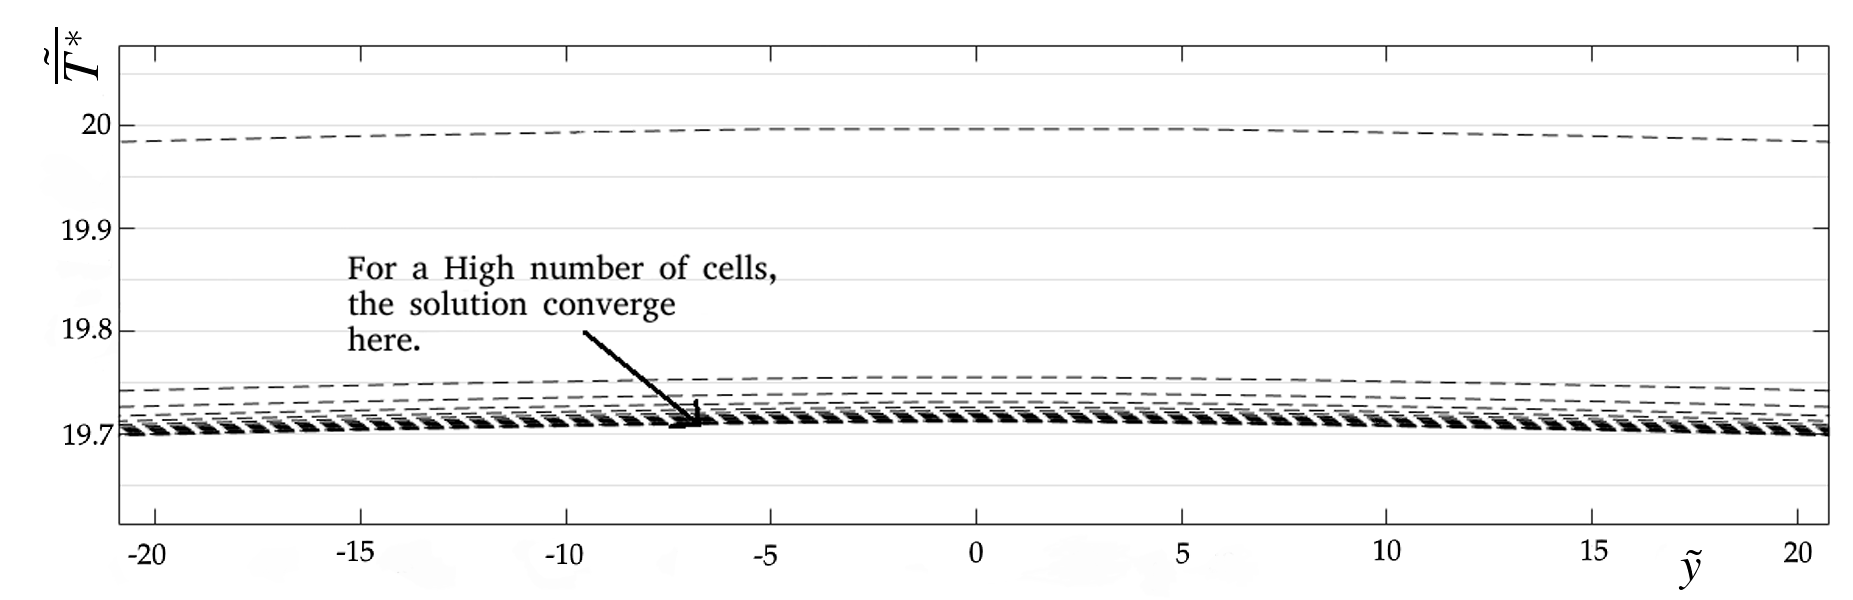
\includegraphics[angle=0, trim={10mm 00mm 0mm 0mm}, clip , scale=0.32]{fotos_formatacao_final/convergnciaprimeira}
	\caption{Convergência do modelo para 400 células.}
	\label{sistema}
\end{figure}